%-*- coding: UTF-8 -*-
\documentclass[hpyerref,UTF8,a4paper,titlepage,12pt,oneside]{ctexbook}
\usepackage{hyperref}
\usepackage{geometry}
\usepackage{xeCJK, fontspec, xunicode, xltxtra,ulem}
\usepackage{amsthm}
\usepackage{amsmath}
\usepackage{amssymb}
\usepackage{mathrsfs}
\usepackage{mathtools}
\usepackage{commath}
\usepackage{listings}
\usepackage{float}
\usepackage{xcolor}
\usepackage{mdframed}

% \graphicspath{{../images/}}
\geometry{a4paper,bottom=2cm}

\title{Qiaternions and Rotation}
\author{陈国庆}
\date{\today}

\bibliography{plain}

% 定理结构
\theoremstyle{definition}
\newtheorem{definition}{定义}[section]
\newtheorem{theorem}{定理}[section]
\newtheorem{corollary}{推论}[theorem]
\newtheorem{lemma}[theorem]{Lemma}
\renewcommand\qedsymbol{$\blacksquare$}

\begin{document}

\maketitle
% \tableofcontents

\section{三维空间旋转}

平面上向量绕原点旋转一个角度,可通过向量与单位复数的乘积来表示,比如向量$v= [x,y]$,逆时针旋转$\theta$后的项链可表示为,
$$
	v^\prime = (x + iy)\cdot (\cos \theta + i\sin\theta)
$$

展开结果又可以表示为$2\times 2$矩阵,
$$
	v^\prime = \begin{bmatrix}
		\cos\theta,& -\sin\theta\\
		\sin\theta,& \cos\theta
	\end{bmatrix}
	\begin{bmatrix}
		x\\
		y
	\end{bmatrix}
$$

这也是线性代数里的结果,上述矩阵称为\textit{旋转矩阵}。\\

三维空间中,绕$z$轴旋转,相当于只改变$xy$而$z$值不变,对应的矩阵为,
$$
	R_z(\theta) = \begin{bmatrix}
			&\cos\theta,&-\sin\theta, & 0\\
			&\sin\theta,&\cos\theta, &0\\
			&0,&0,&1
		\end{bmatrix}
$$

对应的,在$zx$平面绕$y$轴旋转,
$$
	R_y(\theta) = \begin{bmatrix}
			&\cos\theta,&0, &\sin\theta\\
			&0, &1,&0\\
			&-\sin\theta,&0,&\cos\theta\\
		\end{bmatrix}
$$
以及,在$yz$平面绕$x$轴旋转,
$$
	R_x(\theta) = \begin{bmatrix}
			&1,	&0,			&0\\
			&0, &\cos\theta,&-\sin\theta\\
			&0,	&\sin\theta,&\cos\theta\\
		\end{bmatrix}
$$
 
很快发现,$R_y$与$R_x,R_z$对称性并不相同,这是为什么呢?\\

这主要是我们默认用了\textit{右手坐标系},假定逆时针是沿着$x-y-z-x$的顺序,所以$zx$平面相对$z$轴旋转$\theta$,相当于$xz$平面相对$x$轴旋转$-\theta$。

\begin{figure}[H]
	\begin{center}
		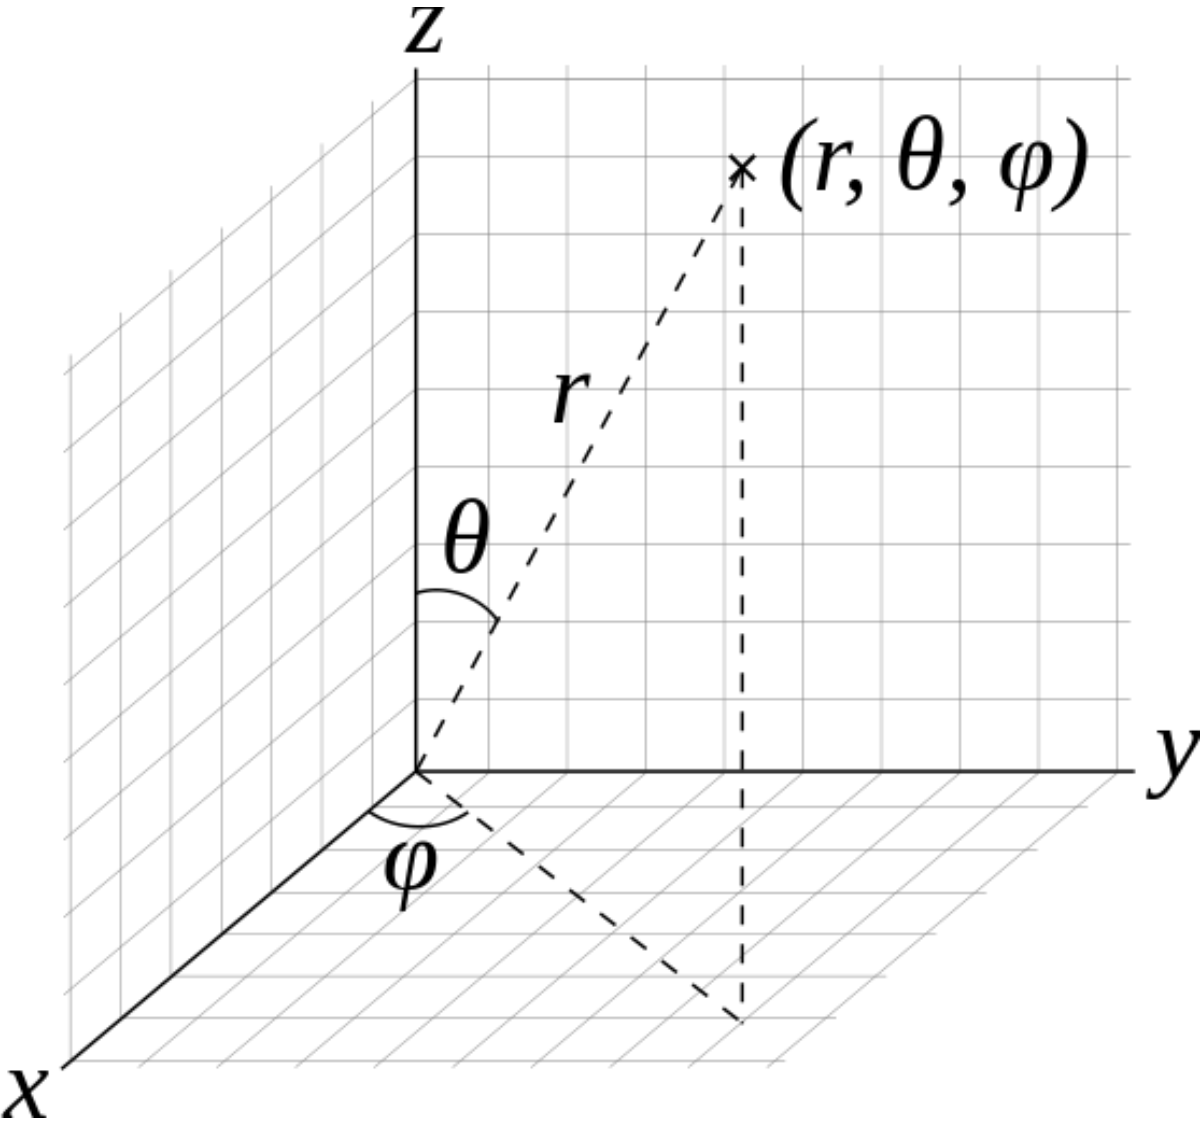
\includegraphics[width=0.8\textwidth]{./images/righthandless.png}
		\caption{右手坐标系}
	\end{center}
\end{figure}


旋转矩阵是单位正交矩阵,存在一些很好的性质,
$$
	R^{-1} = R^T, \quad R(\theta)R(-\theta) = I,\quad R(-\theta)=R^{-1}(\theta)
$$

那向量$\mathbf{v}$绕单位向量$\mathbf{n}$的旋转该如何表示?\\

\begin{figure}[H]
	\begin{center}
		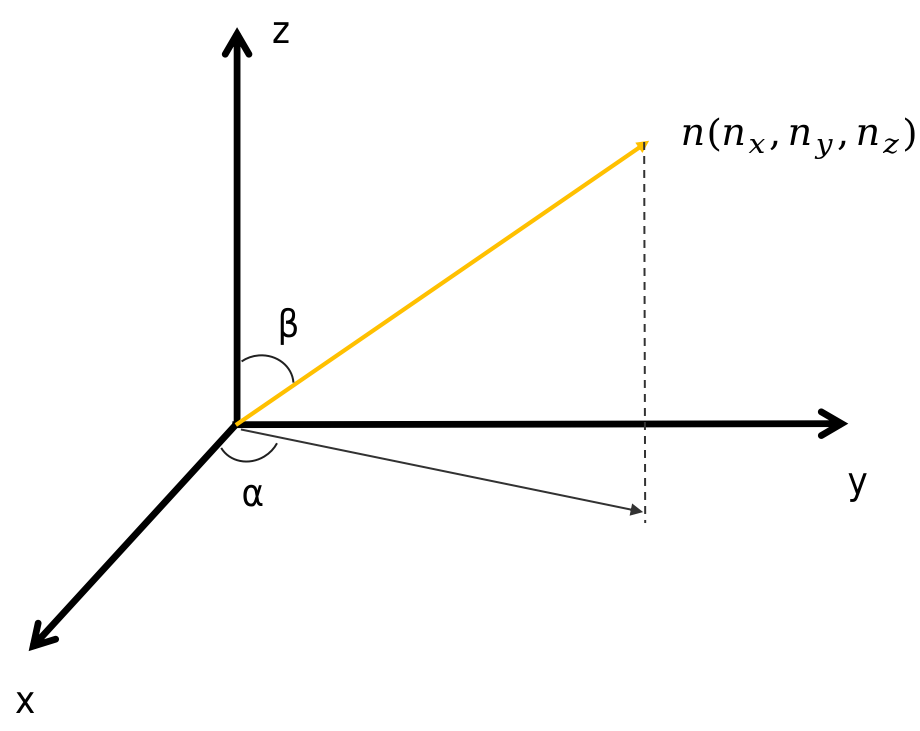
\includegraphics[width=0.8\textwidth]{./images/axis_rotation.png}
	\end{center}
\end{figure}

如上图,分三步操作:
\begin{itemize}
	\item 将$xy$平面绕z轴\textit{逆时针}旋转$\alpha$,再将$zx$平面绕y轴\textit{逆时针}旋转$\beta$,使得$\mathbf{n}$与z轴重合
	\item $\mathbf{v}$绕z轴\textit{逆时针}旋转$\theta$
	\item 将坐标系旋转回原位置
\end{itemize}

如此可直接写出旋转矩阵,
$$
	R_{\mathbf{u}}(\theta) = R_z(\alpha)R_y(\beta)R_z(\theta)R_y(-\beta)R_z(-\alpha)
$$

$\alpha,\beta$可用$\mathbf{n}$的坐标表示,得到最终展开形式,
$$
	R_{\mathbf{u}}(\theta) = \begin{bmatrix}
	&\cos \theta +n_x^2(1-\cos\theta), &n_xn_y(1-\cos\theta)-n_z\sin\theta,&n_xn_z(1-\cos\theta) +n_y\sin\theta\\
	&n_yn_x(1-\cos\theta) + n_x\sin\theta, &\cos\theta + n_y^2(1-\cos\theta),&n_yn_z(1-\cos\theta) - n_x\sin\theta\\
	&n_zn_x(1-\cos\theta) -n_y\sin\theta, &n_xn_y(1-\cos\theta) +n_x\sin\theta,&\cos\theta+n_z^2(1-\cos\theta)
	\end{bmatrix}
$$

将矩阵拆开重新组合可得\textit{罗德里格斯}公式,
$$
	\mathbf{v}^\prime = (1-\cos\theta)(\mathbf{v}\cdot\mathbf{n})\mathbf{n} + \cos\theta\cdot\mathbf{v} + \sin\theta\cdot(\mathbf{n}\times \mathbf{v})
$$

这个看着就舒服多了。\\

我们通过坐标系旋转,一步便得到了3维空间绕固定轴的旋转矩阵,这比一般向量分解来推导容易理解一些。

\section{四元数}
用矩阵表示旋转,二维空间的$2\times 2$矩阵,对应到三维空间是$3\times 3$矩阵,是一个很自然的扩展过程;\\

复数也对应着旋转,是否存在三元复数代表三维空间的旋转?对此,哈密尔顿马上就进行了尝试,引入两个虚数单位,定义了一个三元复数
$$
	\mathbf{v} = v_0 + iv_1 +jv_2
$$

二元复数满足交换律,结合律,当然也期望三元复数也满足这些基本性质,计算一下与另一三元复数$\mathbf{u}$的乘积,
\begin{align*}
	\mathbf{v}\cdot\mathbf{u} 
		&= (v_0 + iv_1 +jv_2)(u_0 + iu_1 +ju_2) \\
		&= v_0u_0 + i(v_0u_1 + v_1u_0) +j(v_0u_2 +v_2u_0) +i^2(v_1u_1) +j^2(v_2u_2) + ij(v_1u_2) + jk(v_2u_1)\\
	\mathbf{u}\cdot\mathbf{v}
		&= (u_0 + iu_1 +ju_2) (v_0 + iv_1 +jv_2)\\
		&= u_0v_0 + i(u_0v_1 + u_1v_0) + j(u_0v_2 + u_2v_0) + i^2(u_1v_1) +j^2(u_2v_2) +ij(u_1v_2) + ji(u_2v_1)
\end{align*}